\section{Versuchsaufbau}
\label{sec:Versuchaufbau}
Der Versuch wird nach dem Schaltplan in Abbildung $\ref{fig:Kreis}$ aufgebaut.

\begin{figure}[H]
  \centering
  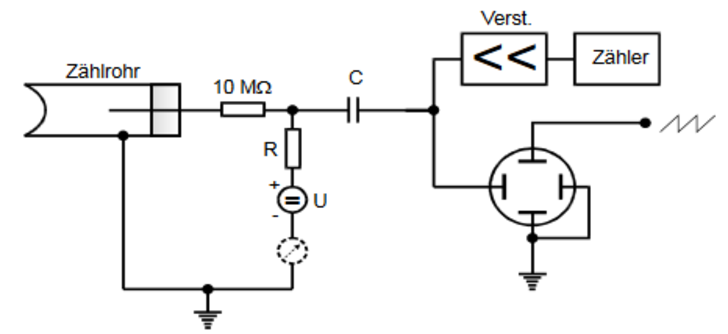
\includegraphics{ressources/Stromkreis.pdf}
  \caption{Skizze der Messapparatur\cite{skript}.}
  \label{fig:Kreis}
\end{figure}

Die an der Anode gesammelte Ladung $Q$  erzeugt im Widerstand $R$ einen Spannungsimpuls, dieser wird im Kondensator entkoppelt. Daraufhin wird der Impuls verstärkt und in dem Zählgerät registriert.
